\documentclass[11pt,a4paper,english]{article}
\usepackage[T1]{fontenc}
\usepackage[utf8]{inputenc}
\usepackage[margin=3cm]{geometry} 	   % Choose your margin here. 
\usepackage{csquotes}
\usepackage{amsmath}
\usepackage{amssymb}
\usepackage{amsbsy}
\usepackage{hyperref}
\usepackage{float}
\usepackage{graphicx}
\usepackage{parskip} 
\usepackage{listings}
\usepackage{booktabs}
\usepackage{caption}
\usepackage{subcaption}
\usepackage[squaren]{SIunits} % Provides SI units like
\lstset{language=Matlab, frame=single, breaklines=true,numbers=left, keywordstyle=\color{blue},rulecolor=\color{black},commentstyle=\color{gray}}
%\usepackage{natbib}
\usepackage{cleveref}
\usepackage{todonotes}
%\usepackage[disable]{todonotes}
\usepackage{listings}
\usepackage[
  backend=bibtex,
  style=numeric,
  isbn=false,
  doi=false]{biblatex}
  
\addbibresource{sources/bibliography.bib}

\definecolor{dkgreen}{rgb}{0,0.6,0}
\definecolor{gray}{rgb}{0.5,0.5,0.5}
\definecolor{pink}{rgb}{0.63, 0.13, 0.94}
\lstset{language=Matlab, 
	keywords={break, case, catch, continue,else,elseif,end,for,function,
		global,if,otherwise,persistent,return,switch,try,while},
	basicstyle=\ttfamily,
	keywordstyle=\color{blue},
	commentstyle=\color{dkgreen},
	stringstyle=\color{pink},
	numbers=left,
	numberstyle=\tiny\color{gray},
	stepnumber=1,
	numbersep=10pt,
	backgroundcolor=\color{white},
	tabsize=4,
	showspaces=false,
    showstringspaces=false}


\title{Guidance and Control of Vehicles}
\author{Group 47 \\ Student 759499 \\Student 759559}
\date{September 2017}

\newcommand{\figref}[1]{\figurename~\ref{#1}}

\begin{document}
\listoftodos 

\begin{titlepage}
    \maketitle
    
    \begin{figure}
    \centering
    \includegraphics[width=0.5\textwidth]{figures/itk_ntnu}\\
    Department of Engineering Cybernetics
    \end{figure}
    \thispagestyle{empty}
\end{titlepage}

% Abstract

\begin{abstract} 


This is our answers and results for Assignment 1. This is a results and discussion text, and not as official as a report would be in presentation, standards and conventions. This text is more about the fact that you as a reader will be able to understand what we have done, what our results were and what we have been able to conclude from them. 

\todo{Ella: Skrev den litt om, men bør den være med ? Den er der nå}
\end{abstract}



\thispagestyle{empty} % Avoid page numbering on the abstract page.

% TOC
\newpage
\tableofcontents
\thispagestyle{empty} % Avoid page numbering on the table of contents.   

\newpage
\setcounter{page}{1}
\setcounter{subsection}{2}

\newpage
\section*{Problem 1 - Attitude Control of Satellite}

The objective of problem 1 is to control attitude of a Satellite. The satellites equations of motions are represented in equation \eqref{eq:dynamics}, equation ?? \todo{find number in fossen} \cite{Fossen2011}. The parameters for this specific Satellite are; $\mathbf{I}_{CG} = mr^2$, $m = 100 kg$, $r = 2.0 m$. 

\begin{subequations}
\label{eq:dynamics}
	\begin{align}
		\dot{\mathbf{q}} = \mathbf{T}_q (\mathbf{q} ) \boldsymbol{\omega} \\
		\mathbf{I}_{CG} \dot{\boldsymbol{\omega}} - \mathbf{S} (\mathbf{I}_{CG} \boldsymbol{\omega} ) \boldsymbol{\omega} & =  \boldsymbol{\tau} \label{eq:omega_dot}
	\end{align}	
\end{subequations}


\todo{Should we write introduction ?}

\subsection*{Problem 1.1: Finding the equilibrium point} 

The equilibrium point is defined as the steady-state solution of a system, meaning $\dot{\mathbf{x}} = 0$ with $\mathbf{x}$ being the state of the system.


The equilibrium point $\mathbf{x_0}$ of the closed-loop system $\mathbf{x} = [ \boldsymbol{\epsilon}^T, \boldsymbol{\omega}^T]^T$ corresponding to $\mathbf{q} = [\eta,\epsilon_1, \epsilon_2, \epsilon_3]^T$ and $\boldsymbol{\tau} = \boldsymbol{0}$ may be found by setting $\boldsymbol{\epsilon} = \mathbf{0}$ and $\dot{\boldsymbol{\omega}} = \mathbf{0}$. The equation for $\boldsymbol{\epsilon}$ and $\boldsymbol{\omega}$ may be found by using equation (2.86) in \cite{Fossen2011} and \eqref{eq:omega_dot}. From equation (2.86) in \cite{Fossen2011} and \eqref{eq:omega_dot} the following equations was found:


\begin{subequations}
\label{eq:dynamics}
	\begin{align}
		\dot{\boldsymbol{\epsilon}} =  (\eta \mathbf{I}_{3X3} + \mathbf{S}(\boldsymbol{\epsilon}) ) \boldsymbol{\omega} \\
		 \dot{\boldsymbol{\omega}} = \mathbf{I}_{CG}^{-1} (\mathbf{S} (\mathbf{I}_{CG} \boldsymbol{\omega} ) \boldsymbol{\omega} +  \boldsymbol{\tau})
	\end{align}	
\end{subequations}







A matrix (and an equation without equation number) can be created as: 
\begin{equation*}	% The star indicates that you don't want to give this equation a number. Normally used if you don't refer to the equation.
	\mathbf{A} = 
	\begin{bmatrix}
		a & b & c \\ d & e & f \\ g & h & i
	\end{bmatrix}
\end{equation*}

\subsection*{Problem 1.2}
Answer Problem 1.2 here. Bold words can be written as \textbf{something bold}. It is also possible to create a new section level:
\subsubsection*{Inner Section 1}
\emph{text..}

\subsubsection*{Inner Section 2}
...

\subsection*{Problem 1.3}
Answer Problem 1.3 here. Equation (2) from the assignment can be written as: 
\begin{equation}
  \label{eq:tau}
  \mathbf{\tau} = -\mathbf{K}_d \boldsymbol{\omega} - k_p \boldsymbol{\epsilon}
\end{equation}

\subsection*{Problem 1.4}
The quaternion error can be written as
 \begin{equation}
	 \tilde{\mathbf{q}} := \left[
	 \begin{array}{c}
		 \tilde{\eta} \\
		 \tilde{\epsilon}
	 \end{array}
	 \right] = \bar{\mathbf{q}}_d \otimes \mathbf{q} 
	 \label{eq:q_tilde}
 \end{equation} 

...

% Note that \mathbf can be used for bold letters in math mode (within equations and dollar signs). \boldsymbol can be used to get bold greek letters.  




\subsection*{Problem 1.5}
For each time iteration, the desired attitude $\mathbf{q}_d(t)$ given by $\phi(t) = 10sin(0.1t), \theta(t) = 0, \psi(t) = 15cos(0.05t)$, was converted to radians and then converted to quaternions by the use of the MATLAB function \texttt{euler2q()}. This was then conjugated and cross multiplied with the current $\mathbf{q}$ iteration by the use of the MATLAB functions \texttt{quatconj()} and \texttt{quatmultiply()} respectively. By doing so, $\mathbf{\tilde{q}}$ was calculated as per equation \eqref{eq:q_tilde}.

The $\tilde{\epsilon}$ part of $\mathbf{\tilde{q}}$ was extracted and combined with $\omega$ to create the state vector and was multiplied with the $\mathbf{K}$ \todo{referer til der K er skrevet!}to create the control input in the same way as in {\color{blue} attitude1.m}. The initial values were kept the same as previously and the $k_p$ and $k_d$ were changed to 10 and 300 respectively. 

\subsubsection*{Simulation results}

The simulation resulted in the plots given in \Cref{fig:sim_attitude2_euler} and \Cref{fig:sim_attitude2_track}.

\begin{figure}
	\centering
	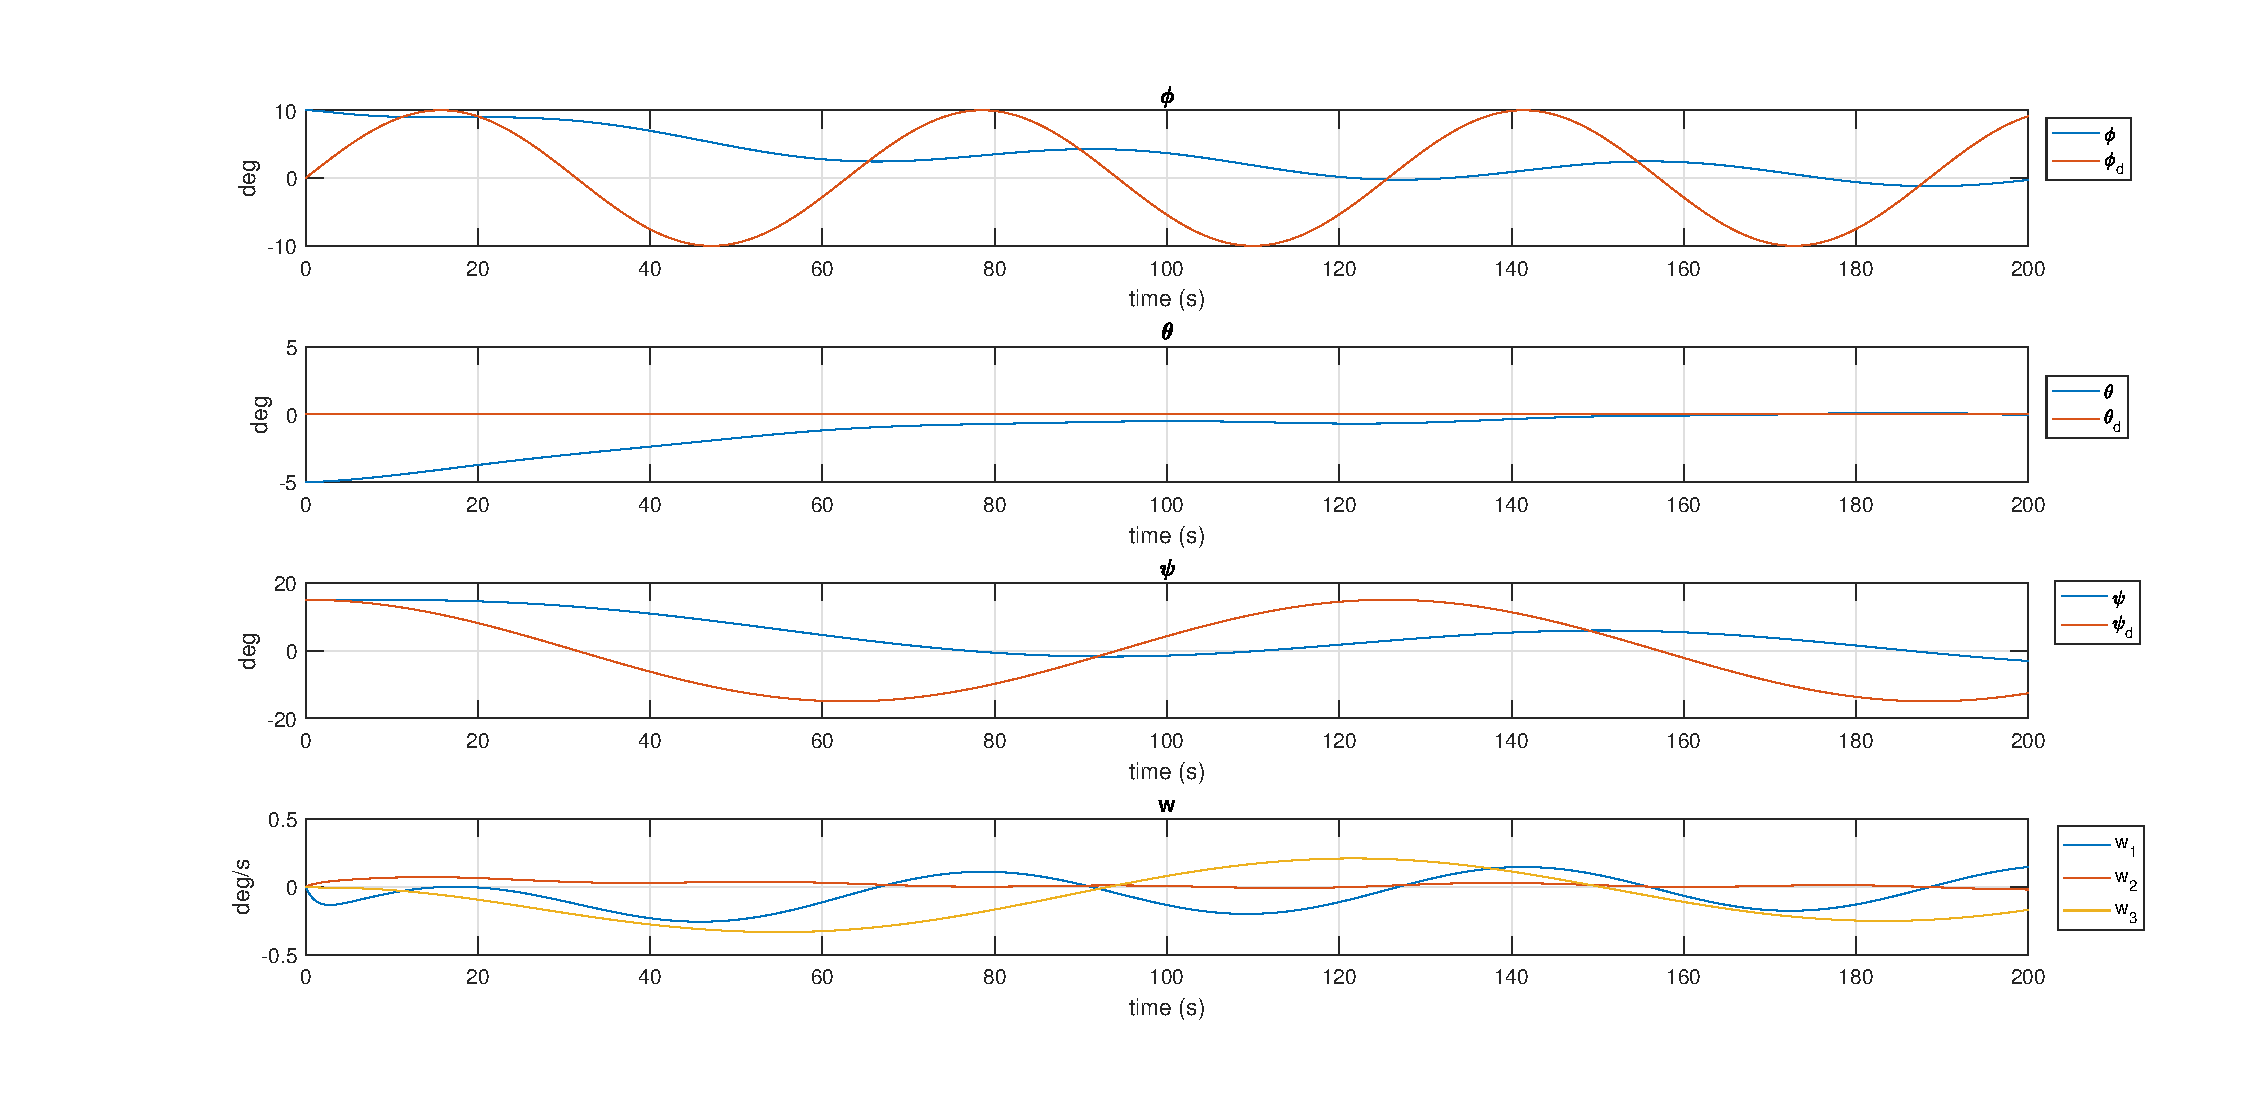
\includegraphics[width=1.00\textwidth]{figures/2_euler.eps}
	\caption{The resulting output euler angles with their corresponding desired values and the resulting output $\omega$ (denoted $\mathbf{w}$ in the plot) from the simulation in attitude2.}
\label{fig:sim_attitude2_euler}
\end{figure}

\begin{figure}
	\centering
	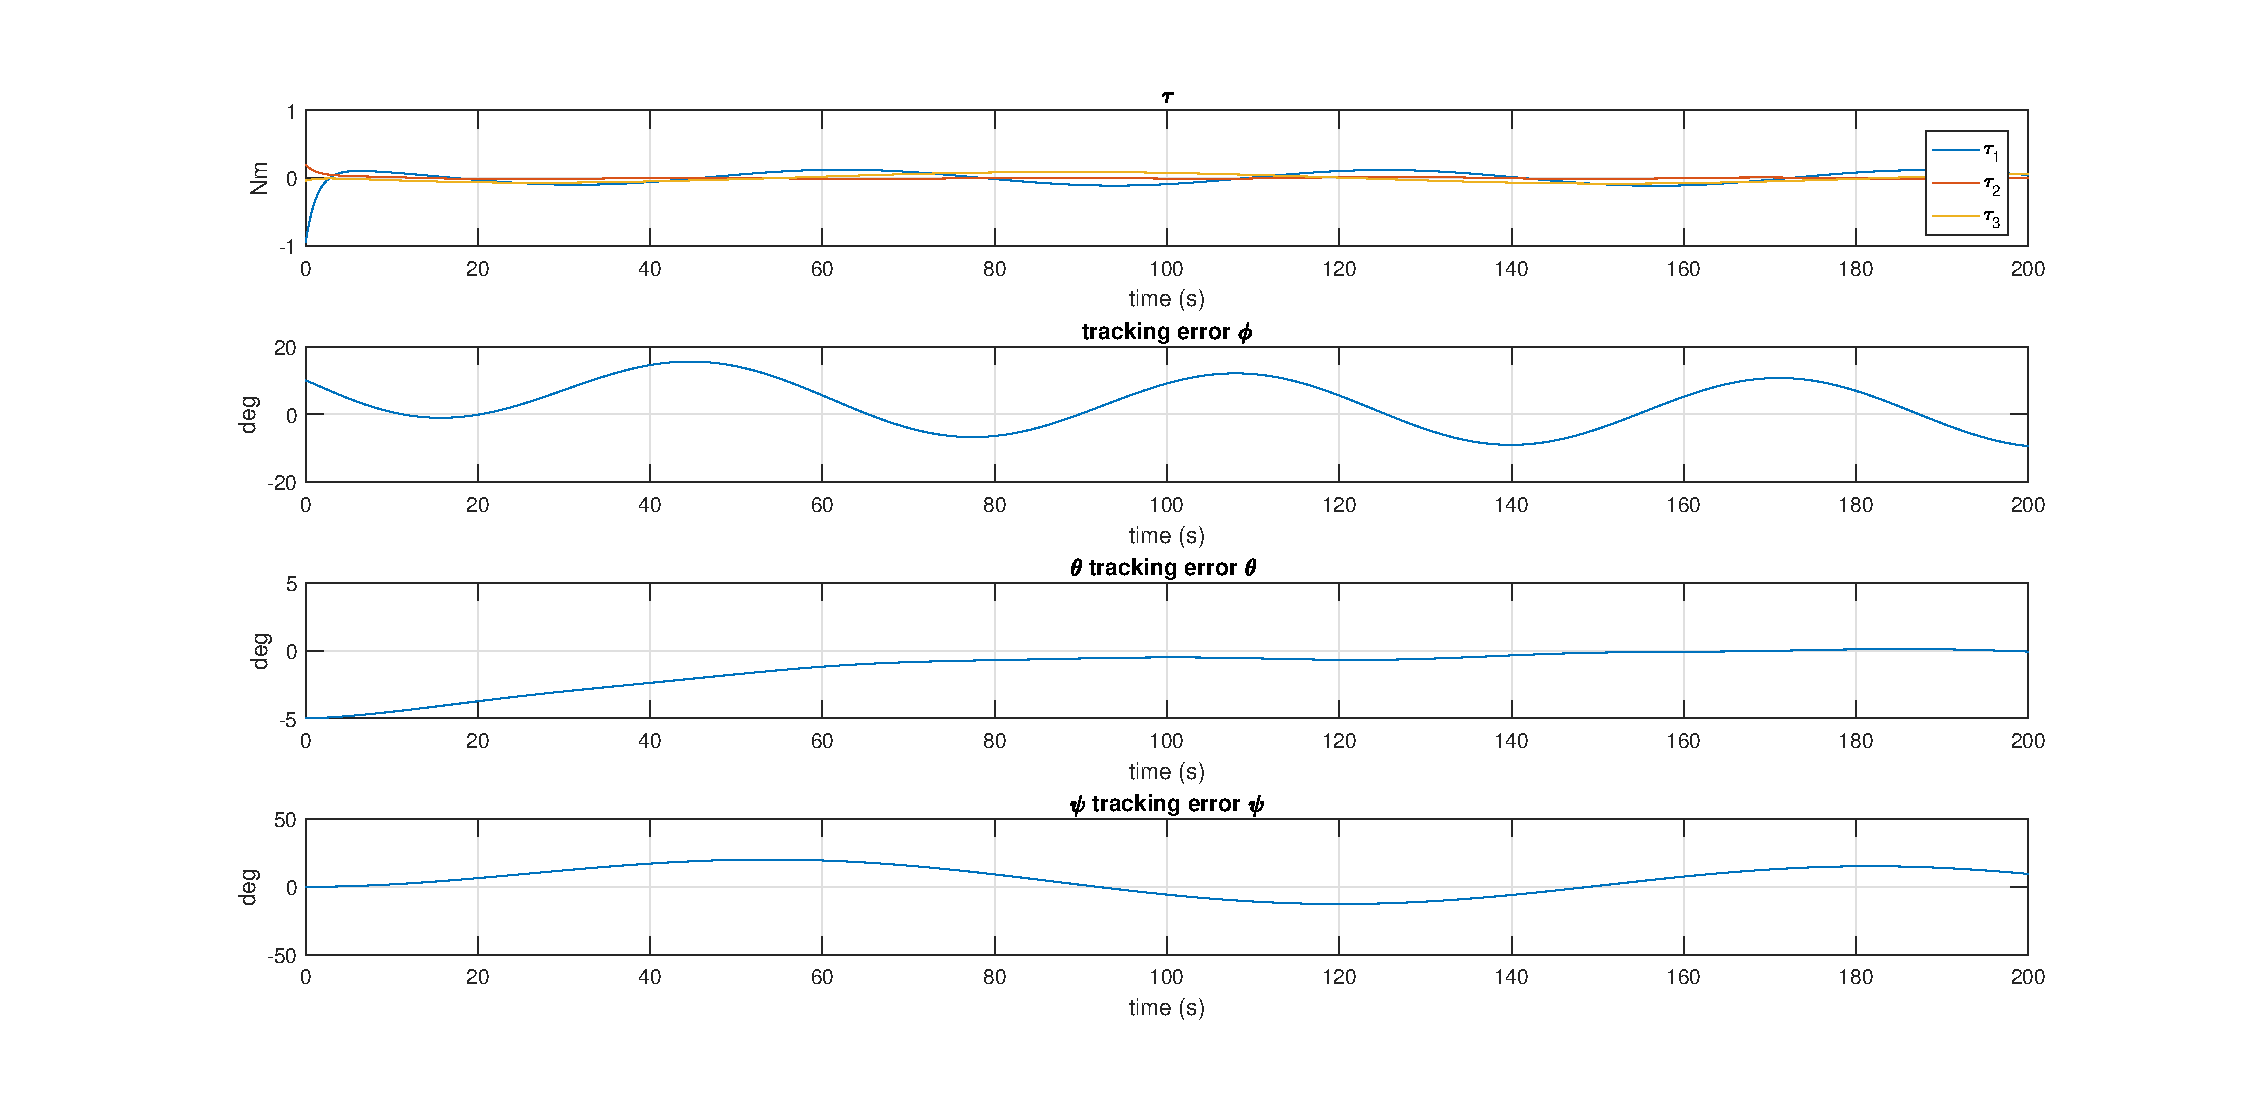
\includegraphics[width=1.00\textwidth]{figures/2_tau_track.eps}
	\caption{ $\tau$, and the tracking errors of the output euler angles from the simulation in attitude2.}
\label{fig:sim_attitude2_track}
\end{figure}

The Figures show that, with the exception of $\theta$, the angles of the satellite are following a sinusoidal pattern as per their desired values. However, they are not in sync with the desired signal and the amplitude is far too low compared to their intended forms, resulting in relatively large sinusoidal tracking errors as can be seen in \Cref{fig:sim_attitude2_track}. One reason for this misbehaviour is the fact that, even though the angles of the satellite is set to move in a specific way, the desired value of $\omega$ is still set to 0. This makes for a contradiction in the controller where neither part is able to do as they are told. The exception is $\theta$ and $\omega_1$ who are both set to 0.

It is also worth mentioning that the $\mathbf{K}$ matrix used for the controller was found using the linearized version of the system. This may also introduce errors.

\subsection*{Problem 1.6}

The attitude control law was modified to:
\begin{equation}
    \tau = -\mathbf{K}_d\tilde{\omega} -k_p\tilde{\epsilon}
    \label{eq:control_law_attitude3}
\end{equation}
\todo{Skal omega være i bold? Det er  ikke det i oppgaveteksten}

with $\tilde{\omega} = \omega - \omega_d$. Differentiating the desired attitude, $\Theta_d$, from the previous problem and calculating $\omega_d$ as

\begin{equation}
    \omega_d = \mathbf{T}_{\Theta_d}^{-1}(\Theta_d)\dot{\Theta_d}
    \label{eq:omega_d}
\end{equation}

We used the MATLAB function \texttt{eulerang()} to get the $\mathbf{T}_{\Theta_d}$ and set $k_p$ and $k_d$ to 10 and 300 respectively as before and used the $\omega_d$ calculated from \eqref{eq:omega_d} in the new simulation {\color{blue} attitude3.m}.

\subsubsection*{Simulation results}

We can see from \Cref{fig:sim_attitude3_euler} and \Cref{fig:sim_attitude3_omega} that the satellite is now able to follow the given reference signal in both angles and angle velocities. From \Cref{fig:sim_attitude3_track} we can see that though there still is an error in the $\phi$ and $\psi$ they are much smaller than previously. Now that $\omega$ and $\epsilon$ have corresponding desired values, they can both be satisfied by the same actions. The cooperation between the two parts of the state, which are in themselves related, is key to making a good controller. The linearization error discussed in the previous problem may still endure and the controller is not exactly the fastest in the galaxy, but all in all the satellite control is much better than before.

\begin{figure}
	\centering
	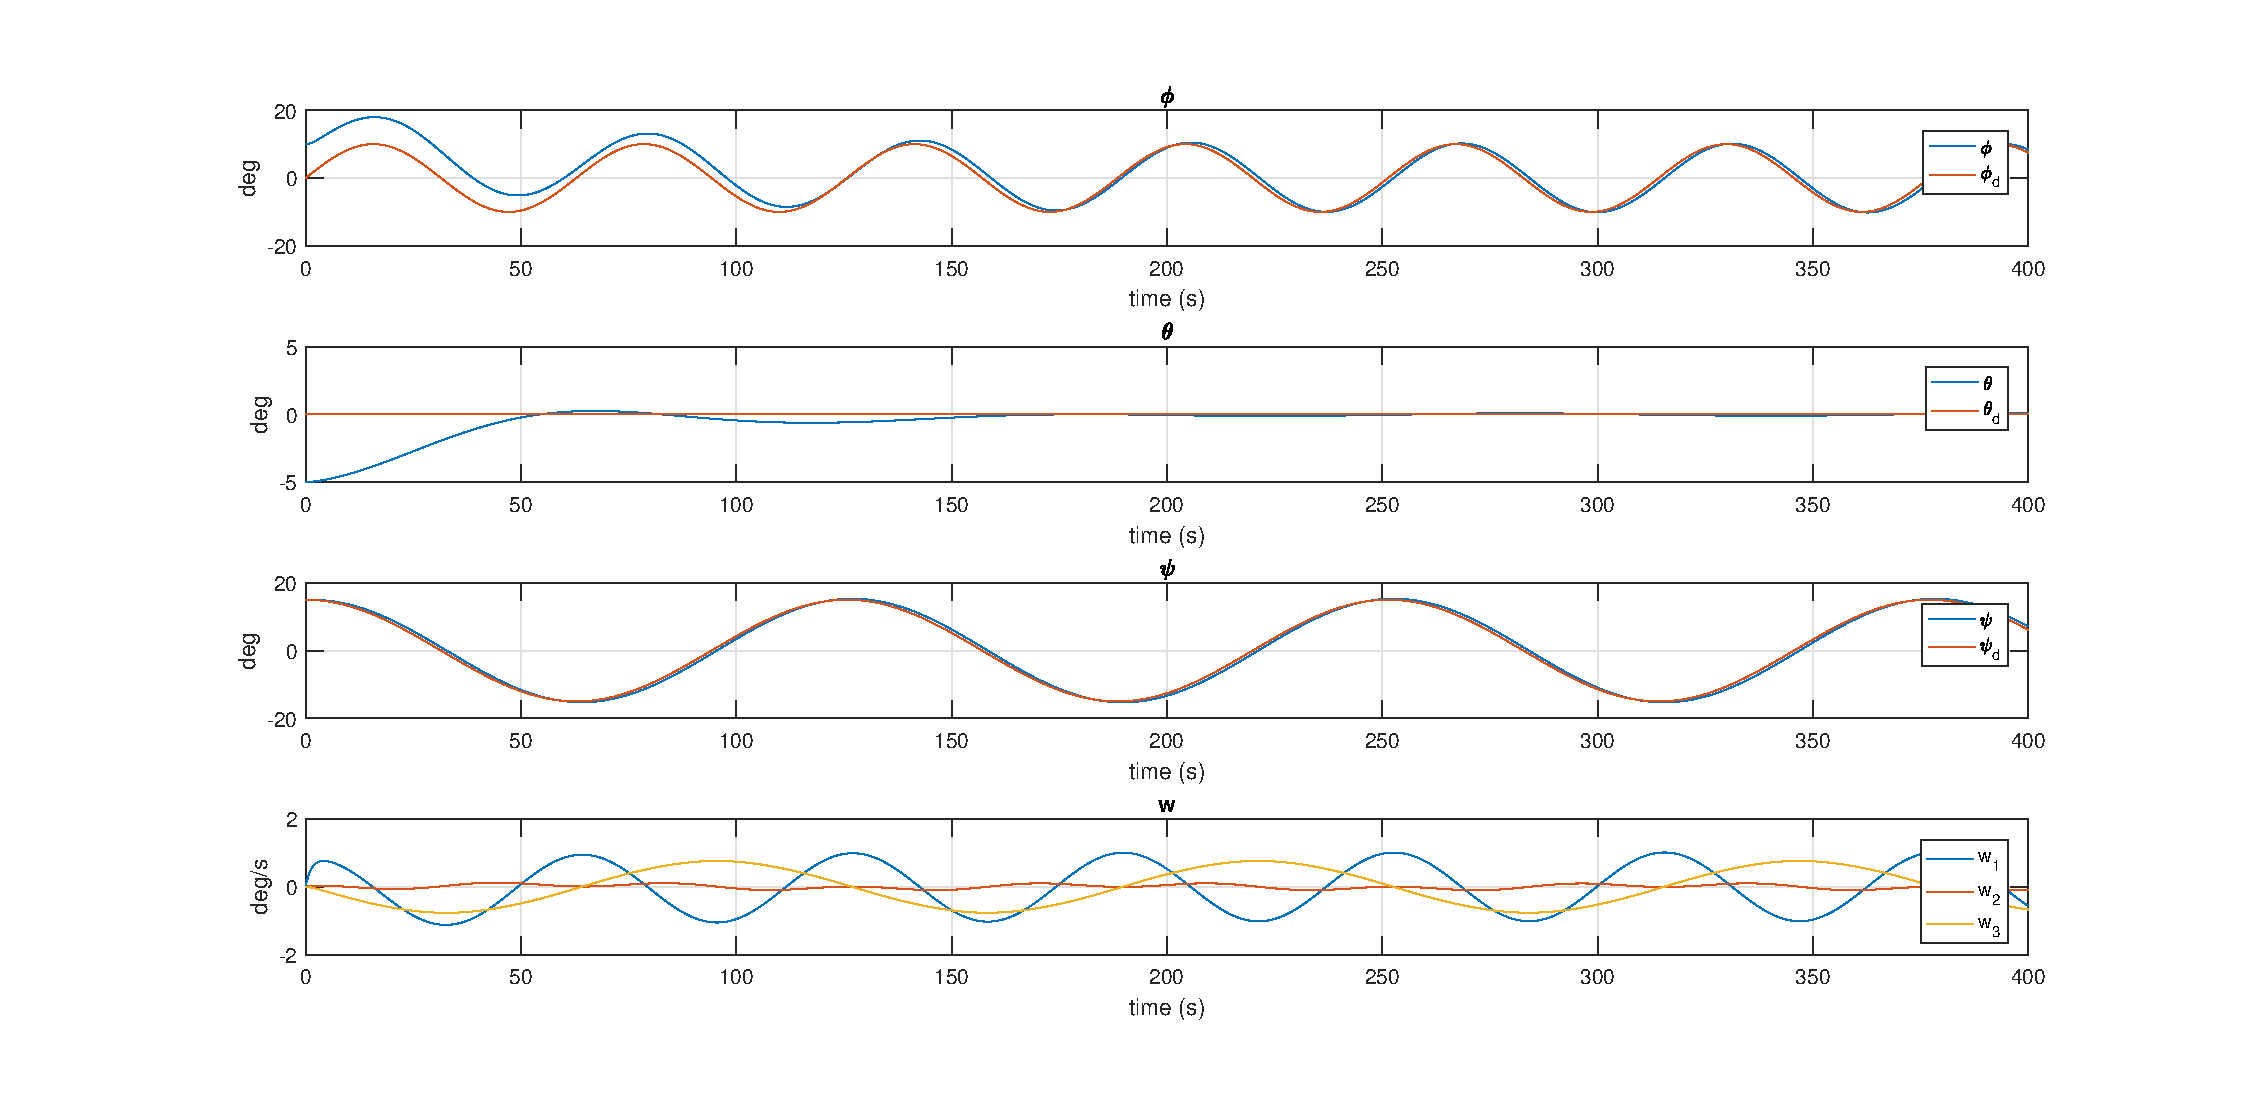
\includegraphics[width=1.00\textwidth]{figures/3_euler.eps}
	\caption{The resulting output euler angles with their corresponding desired values from the simulation in attitude3.}
\label{fig:sim_attitude3_euler}
\end{figure}

\begin{figure}
	\centering
	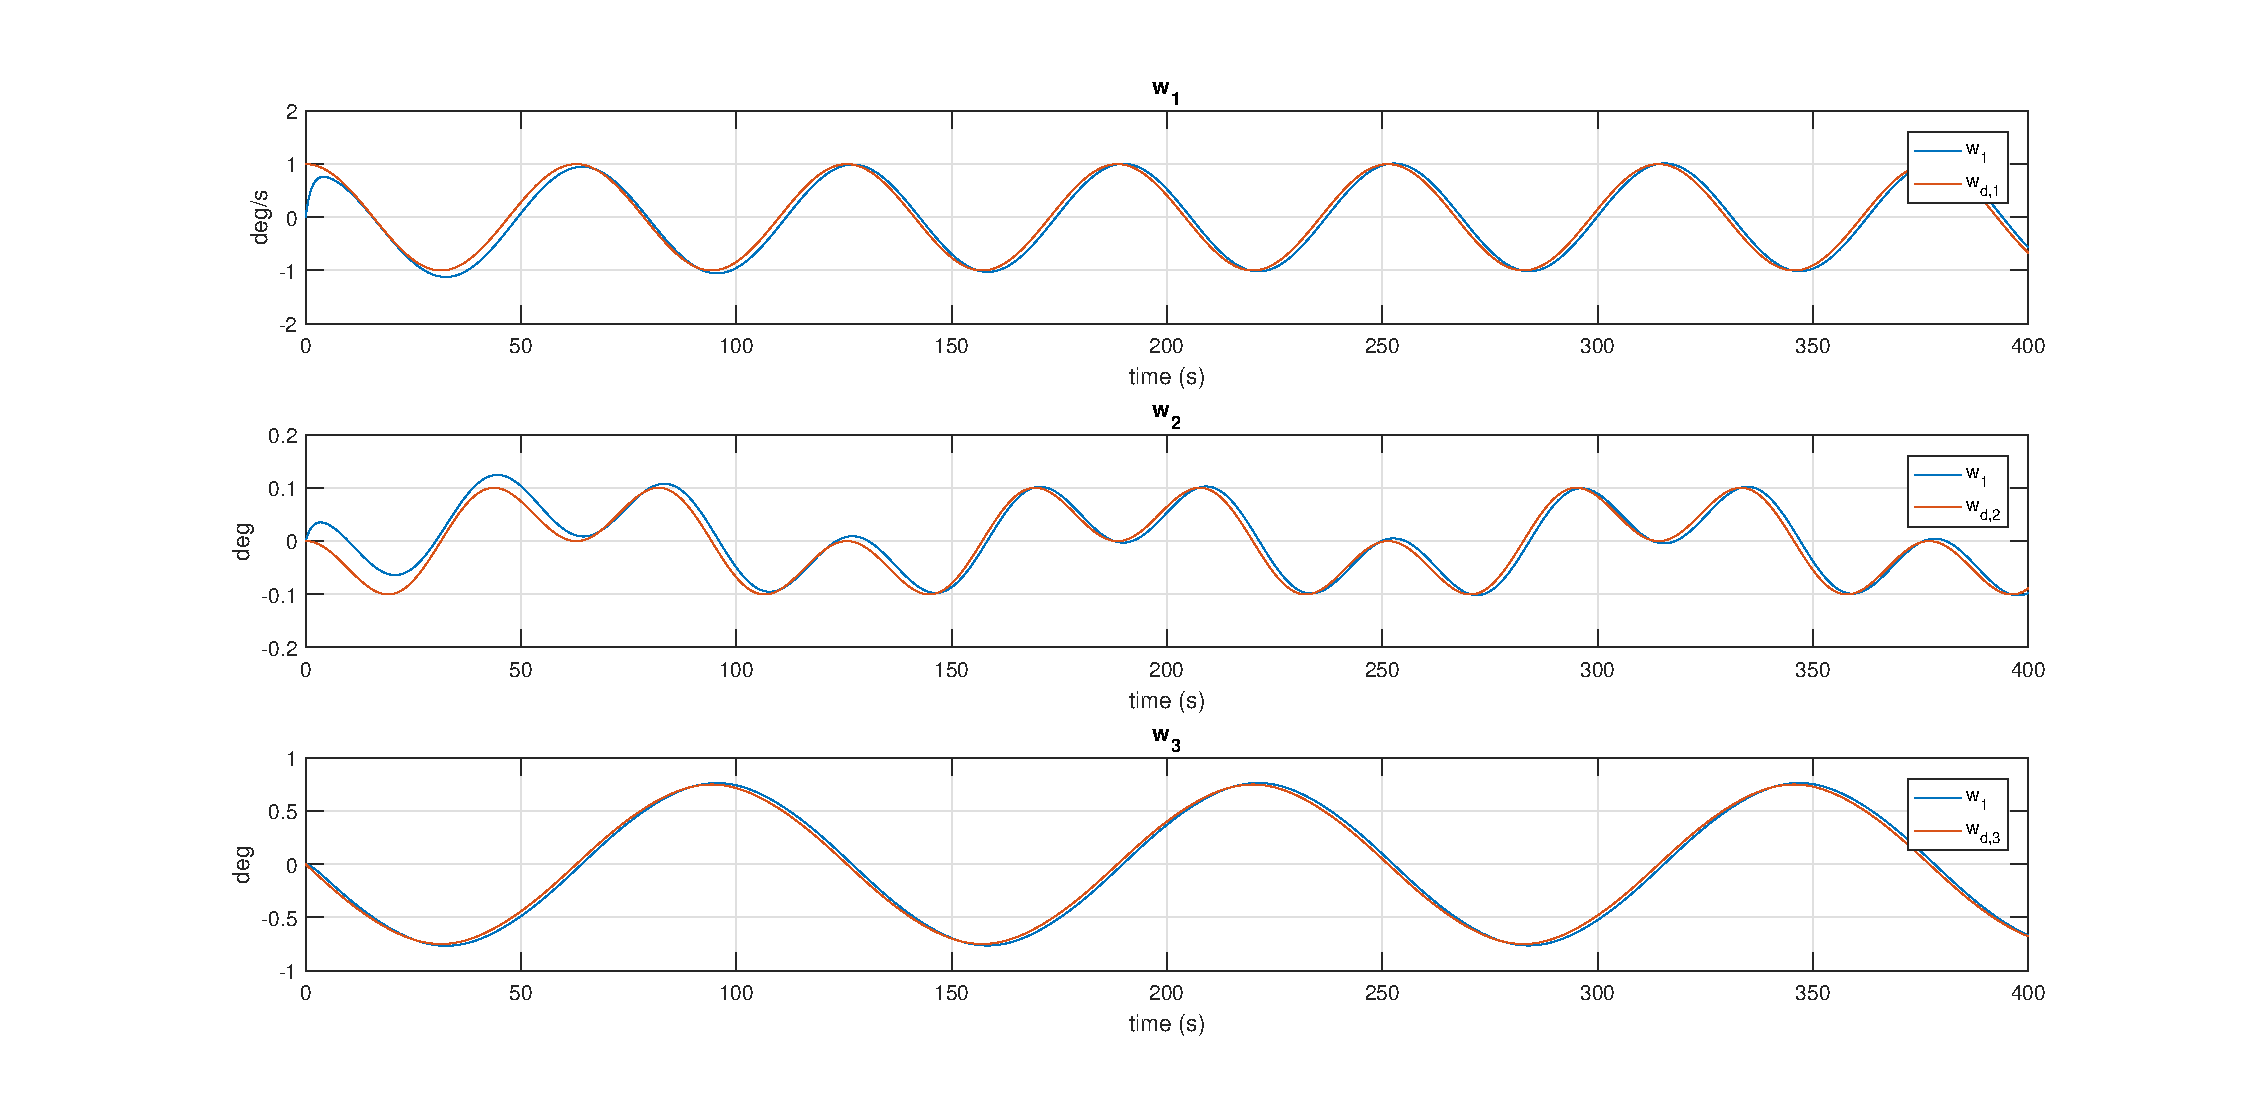
\includegraphics[width=1.00\textwidth]{figures/3_omega.eps}
	\caption{The resulting output $\omega$ (denoted $\mathbf{w}$ in the plots) and the corresponding desired values from the simulation in attitude3.}
\label{fig:sim_attitude3_omega}
\end{figure}

\begin{figure}
	\centering
	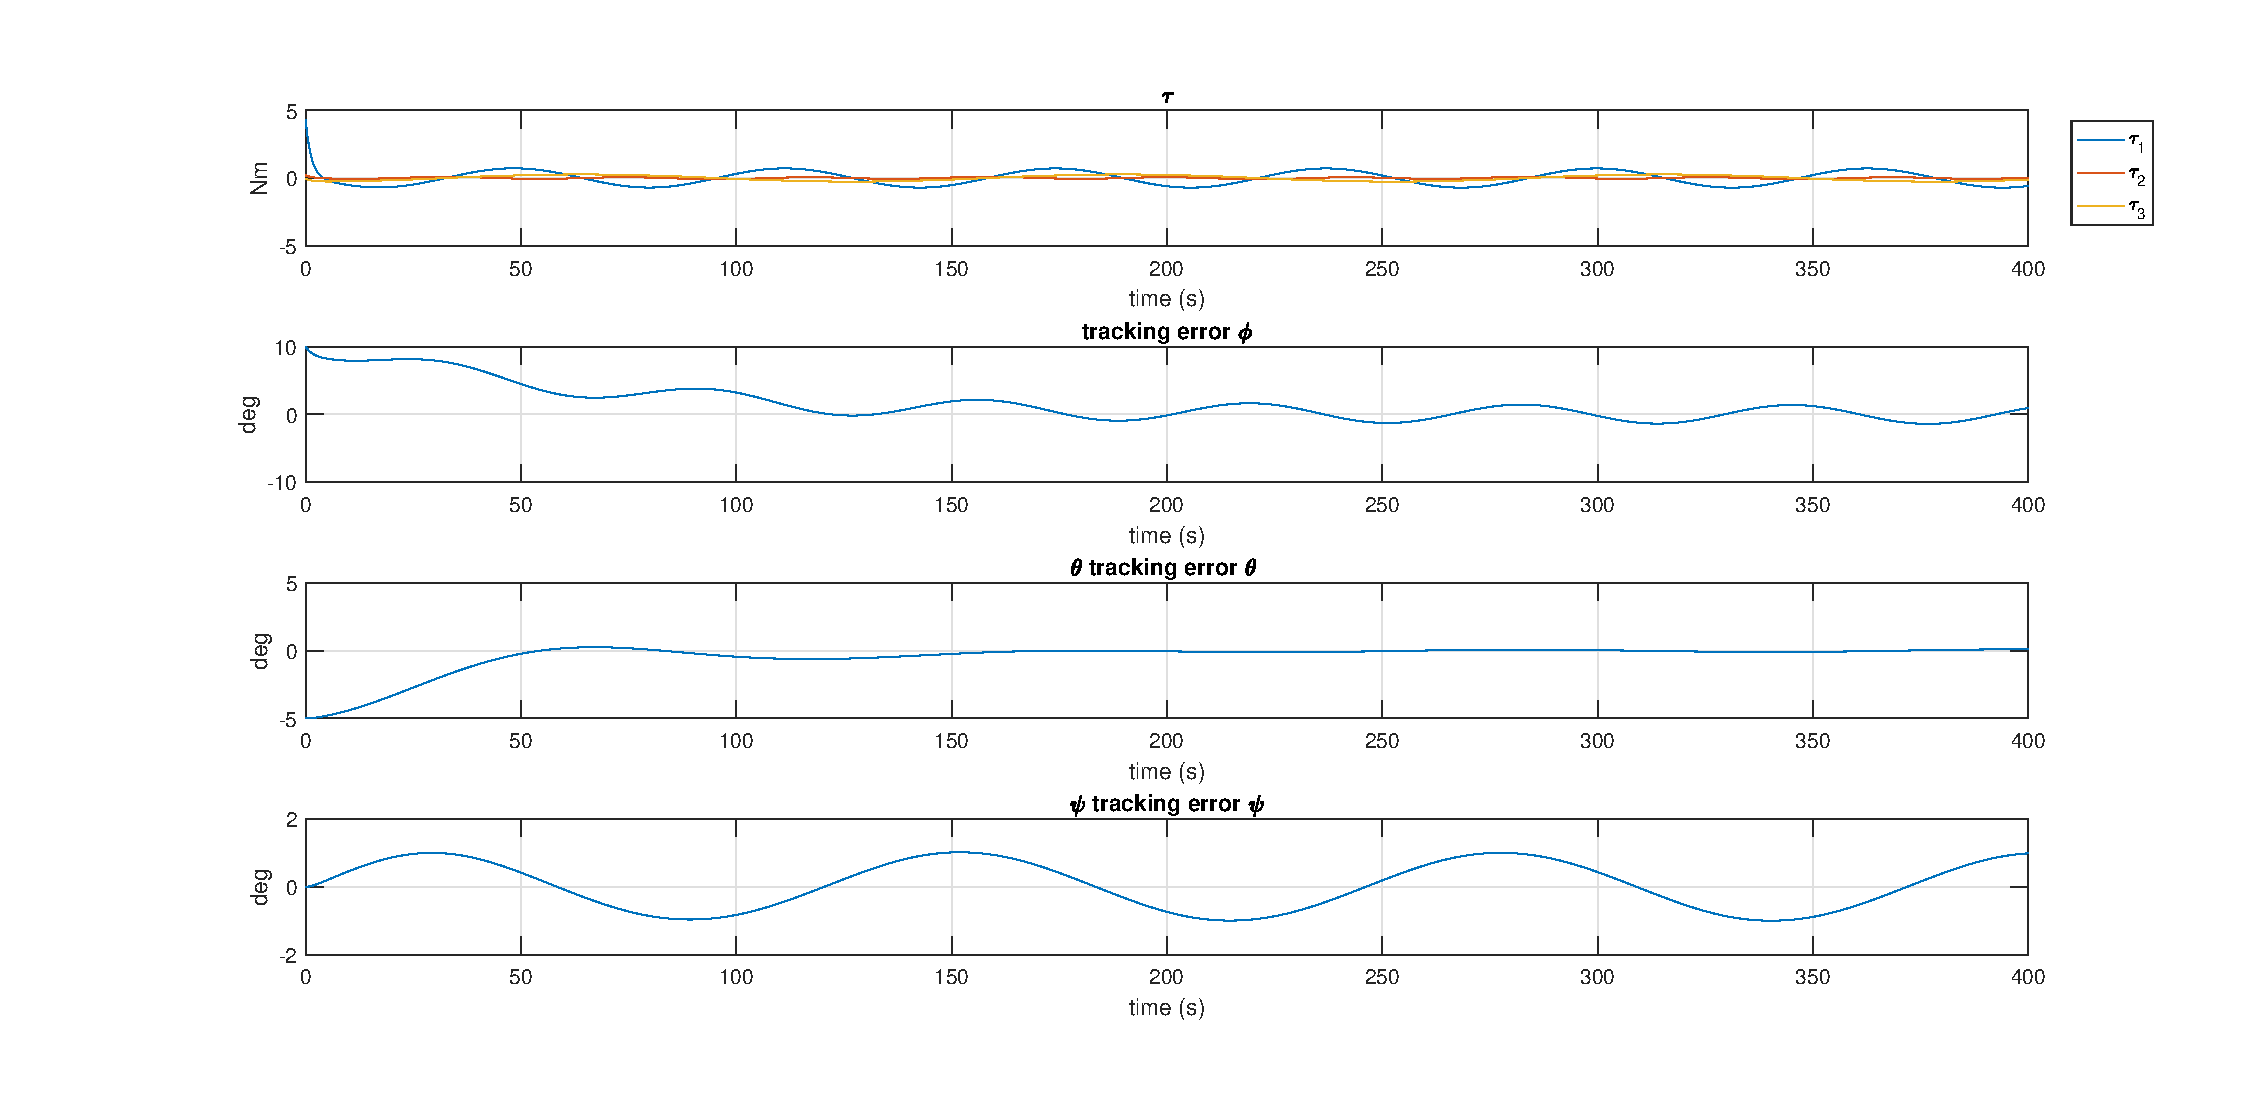
\includegraphics[width=1.00\textwidth]{figures/3_tau_track.eps}
	\caption{ $\tau$, and the tracking errors of the output euler angles from the simulation in attitude3.}
\label{fig:sim_attitude3_track}
\end{figure}

\subsection*{Problem 1.7}
Assuming $\omega_d = 0$ and $\epsilon_d$ and $\eta_d$ constants and the control law given by \eqref{eq:control_law_attitude2}, the Lyapunov function 
 \begin{equation}
	 V = \frac{1}{2} \tilde{\boldsymbol{\omega}}^{\top} \mathbf{I}_{CG}\tilde{\boldsymbol{\omega}} + 2 k_p (1-\tilde{\eta})
 \end{equation}
 
is positive and radially unbounded. 

The reason for its positivity is that $\mathbf{I}_{CG}$ being an identity matrix with a positive number, $mr^2$, on its diagonal, is positive definite. So the first part of V is positive (labeling 0 as a positive number). The second part, consisting of $2 k_p (1-\tilde{\eta})$, may only be negative if $\tilde{\eta} > 1$. This will never happen however, as $\tilde{\eta}$ is part of the unit quaternion $\tilde{q}$ making $|\tilde{\eta}| \leq 1$. Thus the second part of V will also be positive. The Lyapunov function is usually thought of as a representation of the energy in the system so the fact that it is never negative makes sense. 

The function is radially unbounded because as $\tilde{\omega}\rightarrow \infty$ the first part of V, $\frac{1}{2} \tilde{\boldsymbol{\omega}}^{\top} \mathbf{I}_{CG}\tilde{\boldsymbol{\omega}} \rightarrow \infty$

\subsection*{Problem 1.8}
...

% Note that \mathbf can be used for bold letters in math mode (within equations and dollar signs). \boldsymbol can be used to get bold greek letters.  


\section*{Problem 2 - Underwater Vehicles}
Answer Problem 2 in this file. 
\subsection*{Problem 2.1}
Answer problem 2.1 here. The Greek letters for sideslip, crab and course are $\beta_r$, $\beta$ and $\chi$, respectively. The Greek letter for the flight-path angle is $\gamma$.

\subsection*{Problem 2.2}
Answer Problem 2.2 here. The body-fixed velocities can be written as
\begin{equation}
\label{eq:velocity}
	\begin{bmatrix}
		u \\
		v \\
		w
	\end{bmatrix}
	= 
	\begin{bmatrix}
		U \cos( \omega t)\\
		U \sin(\omega t)\\
		0	
	\end{bmatrix}
\end{equation}

\subsection*{Problem 2.3}
Answer Problem 2.3 here.

\subsection*{Problem 2.4}
Answer Problem 2.4 here. Figures can be inserted as:
\begin{figure}[ht]
	\centering
	\includegraphics[width=0.7\textwidth]{assignment_1/rapport/figures/fig1} % Filename is "fig1.png" and must be located in the same folder as this file. If you have a folder containing all the figures you can use "Figures/fig 1" as long as the "Figures" folder is placed in the same folder as this file.
	\caption{Figure of something useful.}
	\label{fig:fig1}
\end{figure}

You can now refer to this figure as \figref{fig:fig1}. You can also insert figures side-by-side:
\begin{figure}[ht]
	\centering
	\begin{subfigure}[b]{0.45\textwidth}
		\includegraphics[width=\textwidth]{assignment_1/rapport/figures/fig1}
		\caption{caption..}
		\label{fig:2a}
	\end{subfigure}
	~ %add desired spacing between images, e. g. ~, \quad, \qquad, \hfill etc. 
	%(or a blank line to force the subfigure onto a new line)
	\begin{subfigure}[b]{0.45\textwidth}
		\includegraphics[width=\textwidth]{assignment_1/rapport/figures/fig1}
		\caption{caption..}
		\label{fig:2b}
	\end{subfigure}
	\begin{subfigure}[b]{0.45\textwidth}
		\includegraphics[width=\textwidth]{assignment_1/rapport/figures/fig1}
		\caption{caption..}
		\label{fig:2c}
	\end{subfigure}
	\begin{subfigure}[b]{0.45\textwidth}
		\includegraphics[width=\textwidth]{assignment_1/rapport/figures/fig1}
		\caption{caption..}
		\label{fig:2d}
	\end{subfigure}		
	\caption{Caption for all figures}\label{fig:2}
\end{figure}

\subsection*{Problem 2.5}
The Nomoto model can be written as
\begin{equation}
	\frac{r}{\delta} (s) = \frac{K}{Ts+1}
\end{equation}
and the equations for the roll and pitch rate as
\begin{equation}
\begin{aligned}
	&\dot{p} + 2\zeta_p\omega_p p + \omega_p^2 \phi = 0\\
	&\dot{q} + 2\zeta_q\omega_q q + \omega_q^2 \theta = 0
\end{aligned}
\end{equation}

\subsection*{Problem 2.6}
References can be placed in the bibliography.bib and referred to as \cite{Fossen2011} and \cite{Fjellstad1994857}.

%\section{Conclusion}\label{sec:conclusion}

In this project, optimal control with and without feedback was implemented on the following in-flight measures of the helicopter under control:
\begin{itemize}
    \item  Pitch/Travel 
    \item  Pitch/Travel and Elevation 
\end{itemize}

The results from this optimization in both cases strongly suggest that the helicopter is controlled better with feedback than without, according to the goal of travelling from $\lambda = \pi $ to $\lambda = 0$. The feedback-less control would have fared somewhat better with a more elaborate and accurate model, ideally taking into account noise as well. The model based errors were somewhat counteracted through feedback, as well as noise such as random winds from surrounding airspace.
The model error because of the dependencies between the angles were one of the most dominant errors, such that it was difficult to have both pitch and travel the optimal planned path.  

During this project we gained practice in formulating a dynamic optimization problem, as well as discretizing and solving the resulting problem using a computer. We gained experience with the implementation and practical use of optimal control with and without feedback.



%\addcontentsline{toc}{section}{Appendix} \label{sec:appendix}
\appendix

\section{MATLAB Code}\label{sec:matlab}

Section contains \texttt{MATLAB}-code this project. Code posted online on BlackBoard are not in the Appendix. 

\subsection{Calculating discrete model, observability matrix and controllability matrix for 4 states} \label{sec:disk_2}
%\lstinputlisting{code/plot_constraint.m}

\begin{lstlisting}[
    language=Matlab,escapechar=|, label={lst:disk_2}, caption={Calculating discrete model for problem 2}]
    %% Model for Ex. 4

    A_c = [ 0 1 0 0 0 0; 
            0 0 -K_2 0 0 0; 
            0 0 0 1 0 0; 
            0 0 -K_1*K_pp -K_1*K_pd 0 0;
            0 0 0 0 0 1; 
            0 0 0 0 -K_3*K_ep -K_3*K_ed ];
    B_c = [ 0 0; 
            0 0; 
            0 0; 
            K_1*K_pp 0;
            0 0; 
            0 K_3*K_ed];
    
    
    %% Forward Euler method
    deltaT = 0.25;
    I = diag([1,1,1,1,1,1]);
    
    A_d = (I + deltaT*A_c);
    B_d = deltaT * B_c;
    
    %% Stabilizible:

    C= ctrb(A_d,B_d)
    rank(C)
    %% Detectable
    
    O = obsv(A_d,C_d)
    rank(O)
    
    %% LQR
    Q = diag([10 2 1 2]);
    R = 1;
    K = dlqr(A_d,B_d,Q,R);   
\end{lstlisting}

\subsection{Calculation of the optimal input sequence with 4 states }

\begin{lstlisting}[
    language=Matlab,escapechar=|, label={lst:main_code_2}, caption={Calculation of the optimal input sequence with 4 states }] 
    
    % TTK4135 - Helicopter lab
    % The code is heavily based on 
    % the hints/template for problem 2.
    % Updated spring 2017, Andreas L. Fl?ten
    
    %% Initialization and model definition
    init; % Init file for our helicopter
    Discrete_model_euler;
    delta_t	= 0.25; % sampling time
    
    % Discrete time system model. x = [lambda r p p_dot]'
    A1 = A_d % From the discrete computation
    B1 = B_d 
    
    % Number of states and inputs
    mx = size(A1,2); % Number of states (number of columns in A)
    mu = size(B1,2); % Number of inputs(number of columns in B)
    
    % Initial values
    x1_0 = pi;                              % Lambda
    x2_0 = 0;                               % r
    x3_0 = 0;                               % p
    x4_0 = 0;                               % p_dot
    x0 = [x1_0 x2_0 x3_0 x4_0]';          % Initial values
    
    % Time horizon and initialization
    N  = 100;                                % Time horizon for states
    M  = N;                                 % Time horizon for inputs
    z  = zeros(N*mx+M*mu,1);                % Initialize z for the whole horizon
    z0 = z;                                 % Initial value for optimization
    
    % Bounds
    ul 	    = -30*pi/180;                   % Lower bound on control - u1
    uu 	    = 30*pi/180;                    % Upper bound on control - u1
    
    xl      = -Inf*ones(mx,1);              % Lower bound on states (no bound)
    xu      = Inf*ones(mx,1);               % Upper bound on states (no bound)
    xl(3)   = ul;                           % Lower bound on state x3
    xu(3)   = uu;                           % Upper bound on state x3
    
    % Generate constraints on measurements and inputs
    [vlb,vub]       = genbegr2(N,M,xl,xu,ul,uu); 
    vlb(N*mx+M*mu)  = 0;                    % We want the last input to be zero
    vub(N*mx+M*mu)  = 0;                    % We want the last input to be zero
    
    % Generate the matrix Q and the vector c (objecitve function weights in the QP problem) 
    Q1 = zeros(mx,mx);
    Q1(1,1) = 1;                             % Weight on state x1
    Q1(2,2) = 0;                            % Weight on state x2
    Q1(3,3) = 0;                             % Weight on state x3 
    Q1(4,4) = 0;                            % Weight on state x4 
    P1 = 1;                                 % Weight on input
    Q = 2*genq2(Q1,P1,N,M,mu);              % Generate Q
    c = zeros(N*mx+M*mu,1);                 % Generate c
    
    %% Generate system matrixes for linear model
    Aeq = gena2(A1,B1,N,mx,mu);           % Generate A
    beq = zeros(M*mx, 1);        	  % Generate b
    beq(1:mx) = A1*x0; % Initial value
    
    %% Solve QP problem with linear model
    tic
    [z,lambda] = quadprog(Q, c, [], [], Aeq, beq, vlb, vub); 
    t1=toc;
    
    % Calculate objective value
    phi1 = 0.0;
    PhiOut = zeros(N*mx+M*mu,1);
    for i=1:N*mx+M*mu
      phi1=phi1+Q(i,i)*z(i)*z(i);
      PhiOut(i) = phi1;
    end
    
    %% Extract control inputs and states
    u  = [z(N*mx+1:N*mx+M*mu);z(N*mx+M*mu)]; |\label{line:extract_vals}| % Control input from solution 
    
    x1 = [x0(1);z(1:mx:N*mx)];              % State x1 from solution
    x2 = [x0(2);z(2:mx:N*mx)];              % State x2 from solution
    x3 = [x0(3);z(3:mx:N*mx)];              % State x3 from solution
    x4 = [x0(4);z(4:mx:N*mx)];              % State x4 from solution
    
    num_variables = 5/delta_t;|\label{line:zero_padding_start}|
    zero_padding = zeros(num_variables,1);
    unit_padding  = ones(num_variables,1);
    
    u   = [zero_padding; u; zero_padding]; 
    x1  = [pi*unit_padding; x1; zero_padding];
    x2  = [zero_padding; x2; zero_padding];
    x3  = [zero_padding; x3; zero_padding];
    x4  = [zero_padding; x4; zero_padding];|\label{line:zero_padding_end}|
    
    %% Plotting
    t = 0:delta_t:delta_t*(length(u)-1); |\label{line:plotting2}|
    input = [t' u]; 
    figure(2)
    hold on;
    subplot(511)
    stairs(t,u),grid
    ylabel('u')
    subplot(512)
    plot(t,x1,'m',t,x1,'mo'),grid
    ylabel('lambda')
    subplot(513)
    plot(t,x2,'m',t,x2','mo'),grid
    ylabel('r')
    subplot(514)
    plot(t,x3,'m',t,x3,'mo'),grid
    ylabel('p')
    subplot(515)
    plot(t,x4,'m',t,x4','mo'),grid
    xlabel('tid (s)'),ylabel('pdot')
\end{lstlisting}

\newpage


\subsection{Calculating controllability, observability matrix and LQR for 6 states }\label{sec:matlab_4_2}

\begin{lstlisting}[
    language=Matlab,escapechar=|, caption={Calculating controllability matrix, observability matrix and LQR for 6 states}, label={lst:matlab_4_2}]

%% Model for Ex. 4
A_c = [0 1 0 0 0 0;
       0 0 -K_2 0 0 0;
       0 0 0 1 0 0;
       0 0 -K_1*K_pp -K_1*K_pd 0 0; 
       0 0 0 0 0 1;
       0 0 0 0 -K_3*K_ep -K_3*K_ed ];
       
B_c = [0 0;
       0 0;
       0 0;
       K_1*K_pp 0;
       0 0;
       0 K_3*K_ed];

%% Forward Euler method
deltaT = 0.25;
I = diag([1,1,1,1,1,1]);

A_d = (I + deltaT*A_c);
B_d = deltaT * B_c;

%% Stabilizable
C = ctrb(A_d,B_d);
rank(C)

%% Detectable
O = obsv(A_d,C_d)
rank(O)

%% Calculate K
Q = diag([20 1 100 2 300000 500]);
R = [1 0; 0 1];
K = dlqr(A_d,B_d,Q,R);   
    
\end{lstlisting}
\newpage

\subsection{Non-linear constraint on elevation }\label{sec:matlab_connstrains}
\begin{lstlisting}[
    language=Matlab,escapechar=|, caption={Non-linear constraint on elevation}]

function [ c, ceq ] = nonlinearconstraints(z)
    
    global N;
    global mx;
    size(N);
    size(mx);
    
    alpha = 0.2;
    beta = 20;
    lambda_t = 2*pi/3;
    c = zeros(N,1);
    for i = 0:(N-1)
        c(i+1) = alpha*exp(-beta*(z(1 +mx*i) - lambda_t)^2) - z(5 +mx*i);
    end

    ceq = [];
    
\end{lstlisting}

\subsection{Calculation of the optimal input sequence with 6 states }\label{sec:matlab_4_3}

\begin{lstlisting} [
    language=Matlab,escapechar=|, label={lst:main_code_4}, caption={Calculation of the optimal input sequence with 6 states}]

% TTK4135 - Helicopter lab
% Hints/template for problem 2.
% Updated spring 2017, Andreas L. Fl?ten

%% Initialization and model definition
init; 
Discrete_model_euler;
delta_t	= 0.25; % sampling time
global N;
global mx;
global M;

% Discrete time system model. 
A1 = A_d; 
B1 = B_d; 

% Number of states and inputs
mx = size(A1,2); % Number of states 
mu = size(B1,2); % Number of inputs

% Initial values
x0 = [ pi 0 0 0 0 0 ]';          

% Time horizon and initialization
N  = 40;            % Time horizon for states
M  = N;             % Time horizon for inputs
z  = zeros(N*mx+M*mu,1);                    
z0 =z; 

% Bounds
pitch_lim = 30*pi/180; |\label{line:start_limit}|
pitch_rate_lim = inf; %20*pi/180;
elevation_lim = inf;
ul =[-pitch_lim; -elevation_lim];
uu =[pitch_lim; elevation_lim];

xl      = [-inf -inf -pitch_lim -pitch_rate_lim -inf -inf]';              % Lower bound on states 
xu      = [inf inf pitch_lim pitch_rate_lim inf inf]';               % Upper bound on states 

% Generate constraints on measurements and inputs
[vlb,vub]       = genbegr2(N,M,xl,xu,ul,uu);|\label{line:end_limit}| ;

% Generate the matrix Q and R and G (objecitve function weights in the QP problem) 
Q1 = diag([1 0 0 0 0 0]);
R = diag([1 1]);
G = 2*genq2(Q1,R,N,M,mu); |\label{line:4_G}|

%% Generate system matrixes for linear model
Aeq = gena2(A1,B1,N,mx,mu) |\label{line:start_eq}|; beq = zeros(M*mx, 1);        
beq(1:mx) = A1*x0 |\label{line:end_eq}|; % Initial value

%% Objective function
f = @(Z) Z'*G*Z;

%% SQP
options = optimoptions('fmincon','Algorithm','sqp','MaxFunEvals',60000);
tic
Z = fmincon(f, z0, [], [], Aeq, beq, vlb, vub, @nonlinearconstraints, options); |\label{line:4_fmincon}|
t1=toc;

%% Extract control inputs and states
u1  = [Z(N*mx+1:mu:N*mx+M*mu); Z(N*mx + M*mu - 1)]; 
u2 = [Z(N*mx+2:mu:N*mx+M*mu); Z(N*mx + M*mu)];


x1 = [x0(1);Z(1:mx:N*mx)];              
x2 = [x0(2);Z(2:mx:N*mx)];              
x3 = [x0(3);Z(3:mx:N*mx)];              
x4 = [x0(4);Z(4:mx:N*mx)];              
x5 = [x0(5);Z(5:mx:N*mx)];              
x6 = [x0(6);Z(6:mx:N*mx)];              

num_variables = 5/delta_t;
zero_padding = zeros(num_variables,1);
unit_padding  = ones(num_variables,1);

u1   = [zero_padding; u1; zero_padding];
u2   = [zero_padding; u2; zero_padding];
u = [u1 u2];
x1  = [pi*unit_padding; x1; zero_padding];
x2  = [zero_padding; x2; zero_padding];
x3  = [zero_padding; x3; zero_padding];
x4  = [zero_padding; x4; zero_padding];
x5  = [zero_padding; x5; zero_padding];
x6  = [zero_padding; x6; zero_padding];
x = [x1 x2 x3 x4 x5 x6];

%% LQR
Q = diag([20 1 100 2 300000 500]);
R = [1 0; 0 1];
K = dlqr(A1,B1,Q,R);      
% 
%% Plotting
t = 0:delta_t:delta_t*(length(u)-1);
input_opt = [t' u]; 
x_opt = [t' x];

\end{lstlisting}



\section{Simulink Diagrams}

\subsection{Diagram from implementation of optimal control of pitch/travel without feedback}

\begin{figure}[!h]
    \centering
	\includegraphics[width=1.2\textwidth]{figures/part2/simulink_lab2.PNG}
	\caption{Simulink diagram for Optimal Control of Pitch/Travel without Feedback}
\label{fig:L2_sim}
\end{figure}

\newpage

\subsection{Diagrams from implementation of optimal control of pitch/travel with feedback}\label{sec:simmulink_3_2}

\begin{figure}[!h]
	\centering
	\includegraphics[width=1.00\textwidth]{figures/part3/im_3_2_full.PNG}
	\caption{Simulink diagram of the system implemented with feedback and LQR-controller.}
    \label{fig:3_2_full}
\end{figure} 

\begin{figure}[!h]
	\centering
	\includegraphics[width=1.00\textwidth]{figures/part3/im_3_2_u.PNG}
	\caption{Feedback implemented in system}
    \label{fig:3_2_u}
\end{figure} 


\newpage

\subsection{Diagram from implementation of optimal control of pitch/travel and elevation with
and without feedback}

\begin{figure}[!h]
    \centering
	\includegraphics[width=1.2\textwidth]{figures/part4/sim_4_open_loop.PNG}
	\caption{Simulink diagram for Optimal Control of Pitch/Travel and Elevation without Feedback}
\label{fig:L4_sim_open}
\end{figure}

\begin{figure}[!h]
    \centering
	\includegraphics[width=1.2\textwidth]{figures/part4/sim_4_closed_loop.PNG}
	\caption{Simulink diagram for Optimal Control of Pitch/Travel and Elevation with Feedback}
\label{fig:L4_sim_closed}
\end{figure}

\begin{figure}[!h]
    \centering
	\includegraphics[width=1.2\textwidth]{figures/part4/sim_4_closed_loop_inside_control.PNG}
	\caption{Inner simulink diagram of the 'Optimal Control' box from \Cref{fig:L4_sim_closed}}
\label{fig:L4_sim_closed_control}
\end{figure}

\newpage

\newpage
\addcontentsline{toc}{section}{References}
\printbibliography
\label{sec:bibliography}


\end{document}
